\section{Ejercicios}

\subsection{Nivel básico}

\begin{ejercicio}

Una fuerza eléctrica realiza un trabajo de

\[
W_e=\SI{0.120}{\joule}
\]

sobre una partícula cargada.

Determine el cambio de energía potencial eléctrica del sistema.

\end{ejercicio}

\begin{respuesta}

\[
\boxed{\Delta U=-\SI{0.120}{\joule}}
\]

\end{respuesta}

\begin{explicacion}

La relación entre el trabajo realizado por la fuerza eléctrica y el cambio de
energía potencial es

\[
\Delta U=-W_e.
\]

Sustituyendo,

\[
\Delta U=-0.120\,\si{\joule}.
\]

Por tanto,

\[
\boxed{\Delta U=-\SI{0.120}{\joule}}.
\]

El campo realizó trabajo positivo, por lo que la energía potencial disminuyó.

\end{explicacion}


\begin{ejercicio}

Dos cargas puntuales

\[
q_1=+\SI{3.0}{\micro\coulomb},
\qquad
q_2=-\SI{2.0}{\micro\coulomb}
\]

están separadas una distancia de

\[
r=\SI{0.40}{\metre}.
\]

Determine la energía potencial eléctrica del sistema, tomando

\[
U(\infty)=0.
\]

\end{ejercicio}

\begin{respuesta}

\[
\boxed{U\approx-\SI{0.135}{\joule}}
\]

\end{respuesta}

\begin{explicacion}

Para dos cargas puntuales,

\[
U=k\frac{q_1q_2}{r}.
\]

No se utiliza valor absoluto porque el signo de las cargas determina el signo de la
energía.

Sustituyendo,

\[
U
=
(8.99\times10^9)
\frac{(3.0\times10^{-6})(-2.0\times10^{-6})}{0.40}.
\]

Por tanto,

\[
\boxed{U\approx-\SI{0.135}{\joule}}.
\]

La energía es negativa porque las cargas tienen signos opuestos.

\end{explicacion}


\begin{ejercicio}

Dos cargas positivas

\[
q_1=+\SI{2.0}{\micro\coulomb},
\qquad
q_2=+\SI{5.0}{\micro\coulomb}
\]

están separadas

\[
r=\SI{0.25}{\metre}.
\]

Determine la energía potencial eléctrica del sistema.

\end{ejercicio}

\begin{respuesta}

\[
\boxed{U\approx+\SI{0.360}{\joule}}
\]

\end{respuesta}

\begin{explicacion}

Aplicamos

\[
U=k\frac{q_1q_2}{r}.
\]

Entonces,

\[
U
=
(8.99\times10^9)
\frac{(2.0\times10^{-6})(5.0\times10^{-6})}{0.25}.
\]

Así,

\[
\boxed{U\approx+\SI{0.360}{\joule}}.
\]

La energía es positiva porque ambas cargas tienen el mismo signo.

\end{explicacion}


\begin{ejercicio}

Dos cargas positivas

\[
q_1=+\SI{2.0}{\micro\coulomb},
\qquad
q_2=+\SI{3.0}{\micro\coulomb}
\]

cambian su separación desde

\[
r_i=\SI{0.60}{\metre}
\]

hasta

\[
r_f=\SI{0.20}{\metre}.
\]

Determine:

\begin{enumerate}
    \item el cambio de energía potencial;
    \item el trabajo realizado por la fuerza eléctrica.
\end{enumerate}

\end{ejercicio}

\begin{respuesta}

\[
\boxed{\Delta U\approx+\SI{0.180}{\joule}}
\]

\[
\boxed{W_e\approx-\SI{0.180}{\joule}}
\]

\end{respuesta}

\begin{explicacion}

El cambio de energía potencial es

\[
\Delta U
=
kq_1q_2
\left(
\frac{1}{r_f}-\frac{1}{r_i}
\right).
\]

Sustituyendo,

\[
\Delta U
=
(8.99\times10^9)
(2.0\times10^{-6})(3.0\times10^{-6})
\left(
\frac{1}{0.20}-\frac{1}{0.60}
\right).
\]

Entonces,

\[
\boxed{\Delta U\approx+\SI{0.180}{\joule}}.
\]

Como

\[
W_e=-\Delta U,
\]

resulta

\[
\boxed{W_e\approx-\SI{0.180}{\joule}}.
\]

Al acercar cargas del mismo signo aumenta la energía potencial del sistema.

\end{explicacion}


\begin{ejercicio}

Dos cargas positivas

\[
q_1=+\SI{4.0}{\micro\coulomb},
\qquad
q_2=+\SI{2.0}{\micro\coulomb}
\]

se encuentran inicialmente infinitamente separadas.

Determine el trabajo que debe realizar un agente externo para acercarlas lentamente
hasta una separación de

\[
r=\SI{0.30}{\metre}.
\]

\end{ejercicio}

\begin{respuesta}

\[
\boxed{W_{\text{ext}}\approx+\SI{0.240}{\joule}}
\]

\end{respuesta}

\begin{explicacion}

En el infinito,

\[
U_i=0.
\]

Al llevar las cargas hasta \(r=\SI{0.30}{\metre}\),

\[
U_f=k\frac{q_1q_2}{r}.
\]

Como el proceso es cuasiestático,

\[
W_{\text{ext}}=\Delta U=U_f-U_i.
\]

Entonces,

\[
W_{\text{ext}}
=
(8.99\times10^9)
\frac{(4.0\times10^{-6})(2.0\times10^{-6})}{0.30}.
\]

Por tanto,

\[
\boxed{W_{\text{ext}}\approx+\SI{0.240}{\joule}}.
\]

El trabajo es positivo porque el agente externo debe vencer la repulsión eléctrica.

\end{explicacion}


\begin{ejercicio}

Una carga

\[
q=+\SI{4.0}{\micro\coulomb}
\]

se desplaza en un campo eléctrico uniforme cuyas componentes son

\[
E_x=\SI{300}{\newton\per\coulomb},
\qquad
E_y=-\SI{200}{\newton\per\coulomb}.
\]

El desplazamiento es

\[
\Delta x=\SI{0.50}{\metre},
\qquad
\Delta y=\SI{0.20}{\metre}.
\]

Determine el trabajo realizado por la fuerza eléctrica y el cambio de energía
potencial.

\end{ejercicio}

\begin{respuesta}

\[
\boxed{W_e=\SI{4.40e-4}{\joule}}
\]

\[
\boxed{\Delta U=-\SI{4.40e-4}{\joule}}
\]

\end{respuesta}

\begin{explicacion}

En un campo uniforme,

\[
W_e=q(E_x\Delta x+E_y\Delta y).
\]

Sustituyendo,

\[
W_e
=
(4.0\times10^{-6})
\left[
(300)(0.50)+(-200)(0.20)
\right].
\]

Entonces,

\[
W_e
=
(4.0\times10^{-6})(150-40)
=
\SI{4.40e-4}{\joule}.
\]

Por tanto,

\[
\boxed{W_e=\SI{4.40e-4}{\joule}}.
\]

El cambio de energía potencial es

\[
\Delta U=-W_e,
\]

por lo que

\[
\boxed{\Delta U=-\SI{4.40e-4}{\joule}}.
\]

\end{explicacion}


\begin{ejercicio}

Una carga positiva se desplaza verticalmente una distancia de

\[
\SI{0.30}{\metre}
\]

en una región donde el campo eléctrico uniforme apunta horizontalmente.

Determine el trabajo realizado por la fuerza eléctrica.

\end{ejercicio}

\begin{respuesta}

\[
\boxed{W_e=0}
\]

\end{respuesta}

\begin{explicacion}

El campo es horizontal y el desplazamiento es vertical.

Por tanto, la fuerza eléctrica y el desplazamiento son perpendiculares.

En componentes rectangulares, si el campo sólo tiene componente \(x\),

\[
E_y=0,
\]

mientras que

\[
\Delta x=0.
\]

Así,

\[
W_e=q(E_x\Delta x+E_y\Delta y)=0.
\]

Por tanto,

\[
\boxed{W_e=0}.
\]

En consecuencia,

\[
\Delta U=0.
\]

\end{explicacion}


\begin{ejercicio}

Dos cargas

\[
q_1=+\SI{5.0}{\micro\coulomb},
\qquad
q_2=-\SI{2.0}{\micro\coulomb}
\]

están separadas

\[
r=\SI{0.25}{\metre}.
\]

Determine el trabajo externo mínimo necesario para separarlas lentamente hasta una
distancia infinita.

\end{ejercicio}

\begin{respuesta}

\[
\boxed{W_{\text{ext}}\approx+\SI{0.360}{\joule}}
\]

\end{respuesta}

\begin{explicacion}

La energía inicial es

\[
U_i=k\frac{q_1q_2}{r}.
\]

Entonces,

\[
U_i
=
(8.99\times10^9)
\frac{(5.0\times10^{-6})(-2.0\times10^{-6})}{0.25}
\approx-\SI{0.360}{\joule}.
\]

En el infinito,

\[
U_f=0.
\]

El trabajo externo cuasiestático es

\[
W_{\text{ext}}=U_f-U_i.
\]

Por tanto,

\[
W_{\text{ext}}
=
0-(-0.360)
=
+\SI{0.360}{\joule}.
\]

Así,

\[
\boxed{W_{\text{ext}}\approx+\SI{0.360}{\joule}}.
\]

\end{explicacion}


\begin{ejercicio}

¿Cuántos términos de interacción deben sumarse para calcular la energía potencial
eléctrica de un sistema formado por cinco cargas puntuales?

\end{ejercicio}

\begin{respuesta}

\[
\boxed{N_{\text{pares}}=10}
\]

\end{respuesta}

\begin{explicacion}

El número de pares diferentes entre \(N\) cargas es

\[
N_{\text{pares}}
=
\frac{N(N-1)}{2}.
\]

Para

\[
N=5,
\]

resulta

\[
N_{\text{pares}}
=
\frac{5(5-1)}{2}
=
10.
\]

Por tanto,

\[
\boxed{N_{\text{pares}}=10}.
\]

Cada interacción debe contarse una sola vez.

\end{explicacion}


\begin{ejercicio}

Una carga fija

\[
Q=+\SI{3.0}{\micro\coulomb}
\]

interactúa con una partícula de carga

\[
q=+\SI{1.0}{\micro\coulomb}
\]

y masa

\[
m=\SI{2.0e-3}{\kilogram}.
\]

La partícula se encuentra inicialmente en reposo a una distancia

\[
r_i=\SI{0.30}{\metre}
\]

y se libera.

Determine su rapidez cuando alcanza una distancia

\[
r_f=\SI{0.60}{\metre}.
\]

\end{ejercicio}

\begin{respuesta}

\[
\boxed{v_f\approx\SI{6.70}{\metre\per\second}}
\]

\end{respuesta}

\begin{explicacion}

Como solamente actúa la interacción eléctrica,

\[
K_i+U_i=K_f+U_f.
\]

La partícula parte del reposo:

\[
K_i=0.
\]

Las energías potenciales son

\[
U_i=k\frac{Qq}{r_i},
\qquad
U_f=k\frac{Qq}{r_f}.
\]

Por tanto,

\[
K_f
=
kQq
\left(
\frac{1}{r_i}-\frac{1}{r_f}
\right).
\]

Sustituyendo,

\[
K_f
=
(8.99\times10^9)
(3.0\times10^{-6})(1.0\times10^{-6})
\left(
\frac{1}{0.30}-\frac{1}{0.60}
\right).
\]

Así,

\[
K_f=\SI{4.495e-2}{\joule}.
\]

Como

\[
K_f=\frac12mv_f^2,
\]

entonces

\[
v_f
=
\sqrt{\frac{2K_f}{m}}.
\]

Sustituyendo,

\[
v_f
=
\sqrt{
\frac{2(4.495\times10^{-2})}{2.0\times10^{-3}}
}.
\]

Por tanto,

\[
\boxed{v_f\approx\SI{6.70}{\metre\per\second}}.
\]

\end{explicacion}


\subsection{Nivel intermedio}

\begin{ejercicio}

Tres cargas ocupan los vértices de un triángulo rectángulo:

\[
q_1=+\SI{2.0}{\micro\coulomb},
\qquad
q_2=-\SI{3.0}{\micro\coulomb},
\qquad
q_3=+\SI{4.0}{\micro\coulomb}.
\]

Las distancias son

\[
r_{12}=\SI{0.30}{\metre},
\qquad
r_{13}=\SI{0.40}{\metre},
\qquad
r_{23}=\SI{0.50}{\metre}.
\]

\begin{center}
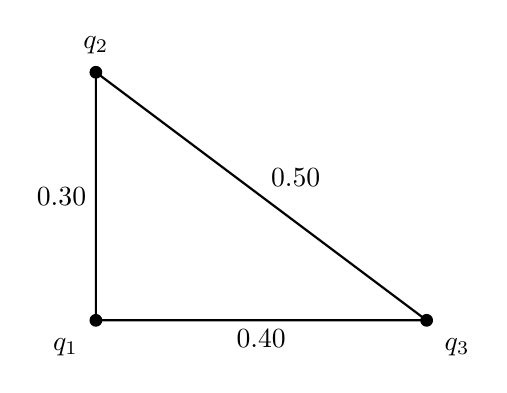
\begin{tikzpicture}[scale=1.05]

\coordinate (A) at (0,0);
\coordinate (B) at (0,3);
\coordinate (C) at (4,0);

\draw[thick] (A) -- (B) -- (C) -- cycle;

\filldraw (A) circle (2pt) node[below left=3pt] {$q_1$};
\filldraw (B) circle (2pt) node[above=3pt] {$q_2$};
\filldraw (C) circle (2pt) node[below right=3pt] {$q_3$};

\node[left] at (0,1.5) {\(\SI{0.30}{\metre}\)};
\node[below] at (2,0) {\(\SI{0.40}{\metre}\)};
\node[above right] at (2,1.5) {\(\SI{0.50}{\metre}\)};

\end{tikzpicture}
\end{center}

Determine la energía potencial eléctrica total.

\end{ejercicio}

\begin{respuesta}

\[
\boxed{U\approx-\SI{0.216}{\joule}}
\]

\end{respuesta}

\begin{explicacion}

Para tres cargas,

\[
U
=
k
\left(
\frac{q_1q_2}{r_{12}}
+
\frac{q_1q_3}{r_{13}}
+
\frac{q_2q_3}{r_{23}}
\right).
\]

Calculamos cada interacción:

\[
U_{12}
=
(8.99\times10^9)
\frac{(2.0\times10^{-6})(-3.0\times10^{-6})}{0.30}
\approx-\SI{0.180}{\joule},
\]

\[
U_{13}
=
(8.99\times10^9)
\frac{(2.0\times10^{-6})(4.0\times10^{-6})}{0.40}
\approx+\SI{0.180}{\joule},
\]

\[
U_{23}
=
(8.99\times10^9)
\frac{(-3.0\times10^{-6})(4.0\times10^{-6})}{0.50}
\approx-\SI{0.216}{\joule}.
\]

Sumamos:

\[
U=U_{12}+U_{13}+U_{23}.
\]

Entonces,

\[
U=-0.180+0.180-0.216.
\]

Por tanto,

\[
\boxed{U\approx-\SI{0.216}{\joule}}.
\]

\end{explicacion}


\begin{ejercicio}

Cuatro cargas iguales

\[
q=+\SI{1.0}{\micro\coulomb}
\]

se encuentran en los vértices de un cuadrado de lado

\[
a=\SI{0.20}{\metre}.
\]

Determine la energía potencial eléctrica del sistema.

\begin{center}
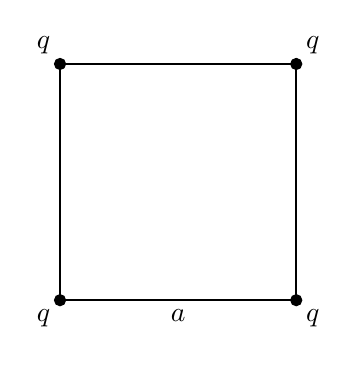
\begin{tikzpicture}[scale=1.0]

\draw[thick] (0,0) rectangle (3,3);

\foreach \p in {(0,0),(3,0),(3,3),(0,3)}
    \filldraw \p circle (2pt);

\node[below left] at (0,0) {$q$};
\node[below right] at (3,0) {$q$};
\node[above right] at (3,3) {$q$};
\node[above left] at (0,3) {$q$};

\node[below] at (1.5,0) {$a$};

\end{tikzpicture}
\end{center}

\end{ejercicio}

\begin{respuesta}

\[
\boxed{U\approx+\SI{0.243}{\joule}}
\]

\end{respuesta}

\begin{explicacion}

Entre cuatro cargas existen seis pares.

En el cuadrado hay cuatro pares separados por una distancia \(a\) y dos pares
diagonales separados por

\[
a\sqrt2.
\]

Por tanto,

\[
U
=
4k\frac{q^2}{a}
+
2k\frac{q^2}{a\sqrt2}.
\]

Factorizamos:

\[
U
=
\frac{kq^2}{a}
\left(
4+\sqrt2
\right).
\]

Sustituyendo,

\[
U
=
\frac{(8.99\times10^9)(1.0\times10^{-6})^2}{0.20}
(4+\sqrt2).
\]

Por tanto,

\[
\boxed{U\approx+\SI{0.243}{\joule}}.
\]

Todas las interacciones son repulsivas, por lo que todos los términos son positivos.

\end{explicacion}


\begin{ejercicio}

Tres cargas están situadas en

\[
q_1=+\SI{1.5}{\micro\coulomb}
\quad\text{en}\quad
(0,0),
\]

\[
q_2=-\SI{2.0}{\micro\coulomb}
\quad\text{en}\quad
(\SI{0.30}{\metre},0),
\]

y

\[
q_3=+\SI{3.0}{\micro\coulomb}
\quad\text{en}\quad
(0,\SI{0.40}{\metre}).
\]

Determine la energía potencial eléctrica total.

\end{ejercicio}

\begin{respuesta}

\[
\boxed{U\approx-\SI{9.66e-2}{\joule}}
\]

\end{respuesta}

\begin{explicacion}

Primero calculamos las distancias.

Entre \(q_1\) y \(q_2\),

\[
r_{12}=\SI{0.30}{\metre}.
\]

Entre \(q_1\) y \(q_3\),

\[
r_{13}=\SI{0.40}{\metre}.
\]

Entre \(q_2\) y \(q_3\),

\[
r_{23}
=
\sqrt{(0.30)^2+(0.40)^2}
=
\SI{0.50}{\metre}.
\]

La energía total es

\[
U
=
k
\left(
\frac{q_1q_2}{r_{12}}
+
\frac{q_1q_3}{r_{13}}
+
\frac{q_2q_3}{r_{23}}
\right).
\]

Sustituyendo,

\[
U
=
(8.99\times10^9)
\left[
\frac{(1.5\times10^{-6})(-2.0\times10^{-6})}{0.30}
+
\frac{(1.5\times10^{-6})(3.0\times10^{-6})}{0.40}
+
\frac{(-2.0\times10^{-6})(3.0\times10^{-6})}{0.50}
\right].
\]

Por tanto,

\[
\boxed{U\approx-\SI{9.66e-2}{\joule}}.
\]

\end{explicacion}


\begin{ejercicio}

Dos cargas

\[
q_1=+\SI{2.0}{\micro\coulomb},
\qquad
q_2=-\SI{5.0}{\micro\coulomb}
\]

cambian su separación desde

\[
r_i=\SI{0.20}{\metre}
\]

hasta

\[
r_f=\SI{0.60}{\metre}.
\]

Determine \(\Delta U\), \(W_e\) y el trabajo externo necesario si el desplazamiento
se realiza lentamente.

\end{ejercicio}

\begin{respuesta}

\[
\boxed{\Delta U\approx+\SI{0.300}{\joule}}
\]

\[
\boxed{W_e\approx-\SI{0.300}{\joule}}
\]

\[
\boxed{W_{\text{ext}}\approx+\SI{0.300}{\joule}}
\]

\end{respuesta}

\begin{explicacion}

Aplicamos

\[
\Delta U
=
kq_1q_2
\left(
\frac{1}{r_f}
-
\frac{1}{r_i}
\right).
\]

Como las cargas tienen signos opuestos,

\[
q_1q_2<0.
\]

Sustituyendo,

\[
\Delta U
=
(8.99\times10^9)
(2.0\times10^{-6})(-5.0\times10^{-6})
\left(
\frac{1}{0.60}
-
\frac{1}{0.20}
\right).
\]

Así,

\[
\boxed{\Delta U\approx+\SI{0.300}{\joule}}.
\]

La energía aumenta porque estamos separando cargas que se atraen.

El trabajo del campo es

\[
W_e=-\Delta U,
\]

por lo que

\[
\boxed{W_e\approx-\SI{0.300}{\joule}}.
\]

Para un desplazamiento lento,

\[
W_{\text{ext}}=\Delta U,
\]

de modo que

\[
\boxed{W_{\text{ext}}\approx+\SI{0.300}{\joule}}.
\]

\end{explicacion}


\begin{ejercicio}

Una carga

\[
q=-\SI{3.0}{\micro\coulomb}
\]

se desplaza en un campo eléctrico uniforme cuyas componentes son

\[
E_x=\SI{400}{\newton\per\coulomb},
\qquad
E_y=\SI{150}{\newton\per\coulomb}.
\]

El desplazamiento es

\[
\Delta x=\SI{0.20}{\metre},
\qquad
\Delta y=-\SI{0.30}{\metre}.
\]

Determine el trabajo eléctrico y el cambio de energía potencial.

\end{ejercicio}

\begin{respuesta}

\[
\boxed{W_e=-\SI{1.05e-4}{\joule}}
\]

\[
\boxed{\Delta U=+\SI{1.05e-4}{\joule}}
\]

\end{respuesta}

\begin{explicacion}

Utilizamos

\[
W_e=q(E_x\Delta x+E_y\Delta y).
\]

Sustituyendo,

\[
W_e
=
(-3.0\times10^{-6})
\left[
(400)(0.20)+(150)(-0.30)
\right].
\]

Dentro del paréntesis,

\[
80-45=35.
\]

Entonces,

\[
W_e
=
(-3.0\times10^{-6})(35)
=
-\SI{1.05e-4}{\joule}.
\]

Por tanto,

\[
\boxed{W_e=-\SI{1.05e-4}{\joule}}.
\]

Como

\[
\Delta U=-W_e,
\]

resulta

\[
\boxed{\Delta U=+\SI{1.05e-4}{\joule}}.
\]

\end{explicacion}


\begin{ejercicio}

Una carga fija

\[
Q=+\SI{4.0}{\micro\coulomb}
\]

interactúa con una partícula de carga

\[
q=+\SI{2.0}{\micro\coulomb}
\]

y masa

\[
m=\SI{5.0e-3}{\kilogram}.
\]

La partícula parte del reposo a

\[
r_i=\SI{0.25}{\metre}.
\]

Determine su rapidez cuando se encuentra a

\[
r_f=\SI{0.75}{\metre}.
\]

\end{ejercicio}

\begin{respuesta}

\[
\boxed{v_f\approx\SI{8.76}{\metre\per\second}}
\]

\end{respuesta}

\begin{explicacion}

La conservación de la energía da

\[
K_i+U_i=K_f+U_f.
\]

Como parte del reposo,

\[
K_i=0.
\]

Por tanto,

\[
K_f
=
kQq
\left(
\frac{1}{r_i}-\frac{1}{r_f}
\right).
\]

Sustituyendo,

\[
K_f
=
(8.99\times10^9)
(4.0\times10^{-6})(2.0\times10^{-6})
\left(
\frac{1}{0.25}
-
\frac{1}{0.75}
\right).
\]

Entonces,

\[
K_f\approx\SI{0.192}{\joule}.
\]

Como

\[
K_f=\frac12mv_f^2,
\]

se obtiene

\[
v_f
=
\sqrt{\frac{2K_f}{m}}.
\]

Así,

\[
\boxed{v_f\approx\SI{8.76}{\metre\per\second}}.
\]

\end{explicacion}


\begin{ejercicio}

Una carga fija

\[
Q=+\SI{3.0}{\micro\coulomb}
\]

interactúa con una partícula

\[
q=-\SI{1.0}{\micro\coulomb}
\]

de masa

\[
m=\SI{1.0e-3}{\kilogram}.
\]

Cuando se encuentra a

\[
r_i=\SI{0.50}{\metre},
\]

la partícula tiene una rapidez

\[
v_i=\SI{4.0}{\metre\per\second}
\]

dirigida hacia la carga fija.

Determine su rapidez cuando alcanza

\[
r_f=\SI{0.20}{\metre}.
\]

\end{ejercicio}

\begin{respuesta}

\[
\boxed{v_f\approx\SI{13.3}{\metre\per\second}}
\]

\end{respuesta}

\begin{explicacion}

Aplicamos conservación de la energía:

\[
\frac12mv_i^2
+
k\frac{Qq}{r_i}
=
\frac12mv_f^2
+
k\frac{Qq}{r_f}.
\]

La energía cinética inicial es

\[
K_i
=
\frac12(1.0\times10^{-3})(4.0)^2
=
\SI{8.0e-3}{\joule}.
\]

La energía potencial inicial es

\[
U_i
=
(8.99\times10^9)
\frac{(3.0\times10^{-6})(-1.0\times10^{-6})}{0.50}
=
-\SI{5.394e-2}{\joule}.
\]

La energía potencial final es

\[
U_f
=
(8.99\times10^9)
\frac{(3.0\times10^{-6})(-1.0\times10^{-6})}{0.20}
=
-\SI{0.13485}{\joule}.
\]

Entonces,

\[
K_f=K_i+U_i-U_f.
\]

Así,

\[
K_f
=
0.0080-0.05394+0.13485
=
\SI{8.891e-2}{\joule}.
\]

Finalmente,

\[
v_f
=
\sqrt{\frac{2K_f}{m}}
\approx\SI{13.3}{\metre\per\second}.
\]

Por tanto,

\[
\boxed{v_f\approx\SI{13.3}{\metre\per\second}}.
\]

\end{explicacion}


\begin{ejercicio}

Una carga

\[
q_1=+\SI{4.0}{\micro\coulomb}
\]

se encuentra a una distancia

\[
r=\SI{0.30}{\metre}
\]

de una carga desconocida \(q_2\).

La energía potencial eléctrica del sistema es

\[
U=-\SI{0.240}{\joule}.
\]

Determine \(q_2\).

\end{ejercicio}

\begin{respuesta}

\[
\boxed{q_2\approx-\SI{2.00}{\micro\coulomb}}
\]

\end{respuesta}

\begin{explicacion}

Partimos de

\[
U=k\frac{q_1q_2}{r}.
\]

Despejamos \(q_2\):

\[
q_2=\frac{Ur}{kq_1}.
\]

Sustituyendo,

\[
q_2
=
\frac{(-0.240)(0.30)}
{(8.99\times10^9)(4.0\times10^{-6})}.
\]

Por tanto,

\[
\boxed{q_2\approx-\SI{2.00}{\micro\coulomb}}.
\]

El signo negativo era esperable porque \(U<0\) y \(q_1>0\).

\end{explicacion}


\begin{ejercicio}

Dos cargas

\[
q_1=+\SI{2.0}{\micro\coulomb},
\qquad
q_2=+\SI{3.0}{\micro\coulomb}
\]

tienen una energía potencial eléctrica

\[
U=\SI{0.180}{\joule}.
\]

Determine la distancia que las separa.

\end{ejercicio}

\begin{respuesta}

\[
\boxed{r\approx\SI{0.300}{\metre}}
\]

\end{respuesta}

\begin{explicacion}

De

\[
U=k\frac{q_1q_2}{r},
\]

despejamos

\[
r=k\frac{q_1q_2}{U}.
\]

Sustituyendo,

\[
r
=
(8.99\times10^9)
\frac{(2.0\times10^{-6})(3.0\times10^{-6})}{0.180}.
\]

Así,

\[
\boxed{r\approx\SI{0.300}{\metre}}.
\]

\end{explicacion}


\begin{ejercicio}

Una carga fija

\[
Q=+\SI{2.0}{\micro\coulomb}
\]

y una partícula de carga

\[
q=+\SI{2.0}{\micro\coulomb}
\]

y masa

\[
m=\SI{2.0e-3}{\kilogram}
\]

se encuentran inicialmente separadas

\[
r_i=\SI{0.40}{\metre}.
\]

La partícula se mueve inicialmente hacia la carga fija con rapidez

\[
v_i=\SI{2.0}{\metre\per\second}.
\]

Determine la distancia mínima a la que puede acercarse.

\end{ejercicio}

\begin{respuesta}

\[
\boxed{r_{\min}\approx\SI{0.383}{\metre}}
\]

\end{respuesta}

\begin{explicacion}

Como las cargas tienen el mismo signo, la partícula se desacelera al acercarse.

En la distancia mínima,

\[
v_f=0,
\]

por lo que

\[
K_f=0.
\]

La energía inicial es

\[
E_{\text{mec}}
=
\frac12mv_i^2
+
k\frac{Qq}{r_i}.
\]

La energía cinética inicial es

\[
K_i
=
\frac12(2.0\times10^{-3})(2.0)^2
=
\SI{4.0e-3}{\joule}.
\]

La energía potencial inicial es

\[
U_i
=
(8.99\times10^9)
\frac{(2.0\times10^{-6})(2.0\times10^{-6})}{0.40}
=
\SI{8.99e-2}{\joule}.
\]

Por tanto,

\[
E_{\text{mec}}
=
0.0040+0.0899
=
\SI{0.0939}{\joule}.
\]

En el punto de máximo acercamiento,

\[
E_{\text{mec}}
=
k\frac{Qq}{r_{\min}}.
\]

Despejando,

\[
r_{\min}
=
\frac{kQq}{E_{\text{mec}}}.
\]

Sustituyendo,

\[
r_{\min}
=
\frac{(8.99\times10^9)(2.0\times10^{-6})(2.0\times10^{-6})}
{0.0939}.
\]

Por tanto,

\[
\boxed{r_{\min}\approx\SI{0.383}{\metre}}.
\]

\end{explicacion}


\subsection{Nivel avanzado}

\begin{ejercicio}

Tres cargas se encuentran en los vértices de un triángulo equilátero de lado \(a\).

Dos de las cargas tienen valor \(+q\) y la tercera tiene valor \(-q\).

Determine la energía potencial eléctrica total del sistema.

\end{ejercicio}

\begin{respuesta}

\[
\boxed{
U=-k\frac{q^2}{a}
}
\]

\end{respuesta}

\begin{explicacion}

Como el triángulo es equilátero, las tres separaciones son iguales:

\[
r_{12}=r_{13}=r_{23}=a.
\]

Supongamos

\[
q_1=q,
\qquad
q_2=q,
\qquad
q_3=-q.
\]

La energía total es

\[
U
=
k
\left(
\frac{q_1q_2}{a}
+
\frac{q_1q_3}{a}
+
\frac{q_2q_3}{a}
\right).
\]

Sustituyendo,

\[
U
=
\frac{k}{a}
\left(
q^2-q^2-q^2
\right).
\]

Por tanto,

\[
\boxed{
U=-k\frac{q^2}{a}
}.
\]

Aunque la carga neta del sistema es \(+q\), la energía total es negativa.

\end{explicacion}


\begin{ejercicio}

Cuatro cargas se encuentran en los vértices de un cuadrado de lado \(a\), alternando
sus signos:

\[
+q,\,-q,\,+q,\,-q.
\]

\begin{center}
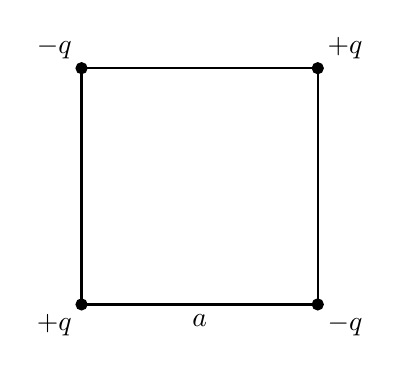
\begin{tikzpicture}[scale=1]

\draw[thick] (0,0) rectangle (3,3);

\filldraw (0,0) circle (2pt) node[below left] {$+q$};
\filldraw (3,0) circle (2pt) node[below right] {$-q$};
\filldraw (3,3) circle (2pt) node[above right] {$+q$};
\filldraw (0,3) circle (2pt) node[above left] {$-q$};

\node[below] at (1.5,0) {$a$};

\end{tikzpicture}
\end{center}

Determine la energía potencial eléctrica total.

\end{ejercicio}

\begin{respuesta}

\[
\boxed{
U=
\frac{kq^2}{a}
\left(
\sqrt2-4
\right)
}
\]

\end{respuesta}

\begin{explicacion}

Los cuatro pares correspondientes a los lados del cuadrado tienen cargas de signos
opuestos.

Cada uno aporta

\[
-\frac{kq^2}{a}.
\]

La contribución total de los lados es

\[
U_{\text{lados}}
=
-\frac{4kq^2}{a}.
\]

Las dos diagonales unen cargas del mismo signo.

La distancia diagonal es

\[
a\sqrt2.
\]

Cada diagonal aporta

\[
\frac{kq^2}{a\sqrt2}.
\]

Las dos diagonales aportan

\[
U_{\text{diag}}
=
\frac{2kq^2}{a\sqrt2}
=
\frac{\sqrt2\,kq^2}{a}.
\]

Por tanto,

\[
U
=
-\frac{4kq^2}{a}
+
\frac{\sqrt2\,kq^2}{a}.
\]

Así,

\[
\boxed{
U=
\frac{kq^2}{a}
\left(
\sqrt2-4
\right)
}.
\]

\end{explicacion}


\begin{ejercicio}

Cuatro cargas iguales \(+q\) se encuentran en los vértices de un cuadrado de lado
\(a\).

Una quinta carga \(Q\) se coloca en el centro.

Determine el valor de \(Q\) para que la energía potencial eléctrica total del sistema
sea cero.

\begin{center}
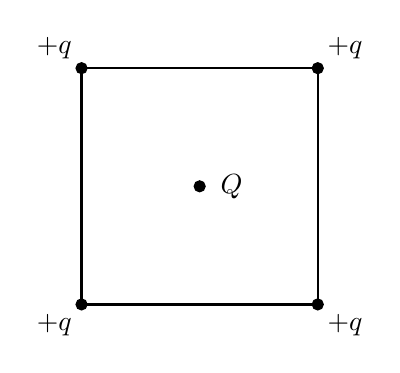
\begin{tikzpicture}[scale=1]

\draw[thick] (0,0) rectangle (3,3);

\filldraw (0,0) circle (2pt) node[below left] {$+q$};
\filldraw (3,0) circle (2pt) node[below right] {$+q$};
\filldraw (3,3) circle (2pt) node[above right] {$+q$};
\filldraw (0,3) circle (2pt) node[above left] {$+q$};

\filldraw (1.5,1.5) circle (2pt)
node[right=4pt] {$Q$};

\end{tikzpicture}
\end{center}

\end{ejercicio}

\begin{respuesta}

\[
\boxed{
Q
=
-\frac{4+\sqrt2}{4\sqrt2}\,q
}
\]

Aproximadamente,

\[
\boxed{Q\approx-0.957\,q}.
\]

\end{respuesta}

\begin{explicacion}

Primero calculamos la energía de las cuatro cargas de los vértices.

Como vimos para un cuadrado,

\[
U_{\text{vértices}}
=
\frac{kq^2}{a}
(4+\sqrt2).
\]

La distancia del centro a cualquiera de los vértices es

\[
r=\frac{a}{\sqrt2}.
\]

La carga central interactúa con las cuatro cargas \(+q\).

Cada interacción tiene energía

\[
U_{Qq}
=
k\frac{Qq}{a/\sqrt2}
=
\frac{\sqrt2\,kQq}{a}.
\]

Como existen cuatro interacciones,

\[
U_{\text{centro}}
=
\frac{4\sqrt2\,kQq}{a}.
\]

La energía total es

\[
U
=
\frac{k}{a}
\left[
q^2(4+\sqrt2)
+
4\sqrt2\,Qq
\right].
\]

Imponemos

\[
U=0.
\]

Entonces,

\[
q^2(4+\sqrt2)
+
4\sqrt2\,Qq
=0.
\]

Despejando,

\[
Q
=
-\frac{4+\sqrt2}{4\sqrt2}\,q.
\]

Por tanto,

\[
\boxed{
Q
=
-\frac{4+\sqrt2}{4\sqrt2}\,q
}.
\]

Numéricamente,

\[
\boxed{Q\approx-0.957\,q}.
\]

\end{explicacion}


\begin{ejercicio}

Tres cargas iguales

\[
q_1=q_2=q_3=+\SI{2.0}{\micro\coulomb}
\]

se encuentran sobre el eje \(x\) en

\[
x_1=-\SI{0.30}{\metre},
\qquad
x_2=0,
\qquad
x_3=+\SI{0.30}{\metre}.
\]

Las cargas \(q_1\) y \(q_2\) se mantienen fijas y \(q_3\), de masa

\[
m=\SI{1.0e-3}{\kilogram},
\]

se libera desde el reposo.

Determine la rapidez de \(q_3\) cuando se encuentra infinitamente lejos.

\end{ejercicio}

\begin{respuesta}

\[
\boxed{v_\infty\approx\SI{19.0}{\metre\per\second}}
\]

\end{respuesta}

\begin{explicacion}

La interacción entre \(q_1\) y \(q_2\) permanece constante porque ambas cargas están
fijas.

Por tanto, para estudiar el movimiento de \(q_3\) sólo necesitamos las energías de
interacción que involucran a \(q_3\).

Inicialmente,

\[
r_{23}=\SI{0.30}{\metre},
\qquad
r_{13}=\SI{0.60}{\metre}.
\]

La energía potencial asociada con \(q_3\) es

\[
U_i
=
kq^2
\left(
\frac{1}{0.30}
+
\frac{1}{0.60}
\right).
\]

Sustituyendo,

\[
U_i
=
(8.99\times10^9)(2.0\times10^{-6})^2
\left(
\frac{1}{0.30}
+
\frac{1}{0.60}
\right).
\]

Entonces,

\[
U_i=\SI{0.1798}{\joule}.
\]

Cuando \(q_3\) se encuentra infinitamente lejos,

\[
U_f=0.
\]

Como parte del reposo,

\[
K_i=0.
\]

La conservación de la energía da

\[
U_i=K_f.
\]

Por tanto,

\[
\frac12mv_\infty^2
=
0.1798.
\]

Despejando,

\[
v_\infty
=
\sqrt{\frac{2(0.1798)}{1.0\times10^{-3}}}.
\]

Así,

\[
\boxed{v_\infty\approx\SI{19.0}{\metre\per\second}}.
\]

\end{explicacion}


\begin{ejercicio}

Una carga

\[
q=+\SI{2.0}{\micro\coulomb}
\]

se desplaza desde

\[
A=(0,0)
\]

hasta

\[
B=(\SI{0.40}{\metre},\SI{0.30}{\metre})
\]

en un campo eléctrico uniforme cuyas componentes son

\[
E_x=\SI{300}{\newton\per\coulomb},
\qquad
E_y=-\SI{200}{\newton\per\coulomb}.
\]

Considere dos trayectorias:

\begin{enumerate}
    \item directamente de \(A\) a \(B\);
    \item de \(A\) a \(C=(\SI{0.40}{\metre},0)\) y luego de \(C\) a \(B\).
\end{enumerate}

\begin{center}
\begin{tikzpicture}[>=Latex,scale=1]

\draw[->] (-0.5,0) -- (5,0) node[right] {$x$};
\draw[->] (0,-0.5) -- (0,4) node[above] {$y$};

\coordinate (A) at (0,0);
\coordinate (C) at (4,0);
\coordinate (B) at (4,3);

\filldraw (A) circle (2pt) node[below left] {$A$};
\filldraw (C) circle (2pt) node[below] {$C$};
\filldraw (B) circle (2pt) node[above right] {$B$};

\draw[->,thick,dashed] (A) -- (B);
\draw[->,thick] (A) -- (C);
\draw[->,thick] (C) -- (B);

\end{tikzpicture}
\end{center}

Calcule el trabajo eléctrico por ambas trayectorias.

\end{ejercicio}

\begin{respuesta}

Para ambas trayectorias,

\[
\boxed{W_e=\SI{1.20e-4}{\joule}}.
\]

\end{respuesta}

\begin{explicacion}

Para el desplazamiento total,

\[
\Delta x=\SI{0.40}{\metre},
\qquad
\Delta y=\SI{0.30}{\metre}.
\]

Como el campo es uniforme,

\[
W_e=q(E_x\Delta x+E_y\Delta y).
\]

Entonces,

\[
W_e
=
(2.0\times10^{-6})
\left[
(300)(0.40)+(-200)(0.30)
\right].
\]

Así,

\[
W_e
=
(2.0\times10^{-6})(120-60)
=
\SI{1.20e-4}{\joule}.
\]

Ahora analizamos la trayectoria \(A\to C\to B\).

En \(A\to C\),

\[
\Delta x=\SI{0.40}{\metre},
\qquad
\Delta y=0,
\]

por lo que

\[
W_{AC}
=
qE_x\Delta x
=
(2.0\times10^{-6})(300)(0.40)
=
\SI{2.40e-4}{\joule}.
\]

En \(C\to B\),

\[
\Delta x=0,
\qquad
\Delta y=\SI{0.30}{\metre},
\]

por lo que

\[
W_{CB}
=
qE_y\Delta y
=
(2.0\times10^{-6})(-200)(0.30)
=
-\SI{1.20e-4}{\joule}.
\]

Entonces,

\[
W_{ACB}
=
W_{AC}+W_{CB}
=
2.40\times10^{-4}
-
1.20\times10^{-4}.
\]

Por tanto,

\[
\boxed{W_{ACB}=\SI{1.20e-4}{\joule}}.
\]

Las dos trayectorias producen el mismo trabajo, como corresponde a una fuerza
electrostática conservativa.

\end{explicacion}


\begin{ejercicio}

La energía potencial de una interacción depende de la separación \(r\) según

\[
U(r)=\frac{A}{r},
\]

donde

\[
A=\SI{0.060}{\joule\metre}.
\]

Determine la fuerza radial cuando

\[
r=\SI{0.30}{\metre}.
\]

Indique si la interacción es atractiva o repulsiva.

\end{ejercicio}

\begin{respuesta}

\[
\boxed{F_r\approx+\SI{0.667}{\newton}}
\]

La interacción es repulsiva.

\end{respuesta}

\begin{explicacion}

La fuerza radial se obtiene a partir de

\[
F_r=-\frac{dU}{dr}.
\]

Como

\[
U(r)=Ar^{-1},
\]

entonces

\[
\frac{dU}{dr}
=
-Ar^{-2}
=
-\frac{A}{r^2}.
\]

Por tanto,

\[
F_r
=
-\left(-\frac{A}{r^2}\right)
=
\frac{A}{r^2}.
\]

Sustituyendo,

\[
F_r
=
\frac{0.060}{(0.30)^2}
=
\SI{0.667}{\newton}.
\]

Así,

\[
\boxed{F_r\approx+\SI{0.667}{\newton}}.
\]

El signo positivo indica que la fuerza apunta hacia valores crecientes de \(r\), es
decir, corresponde a una interacción repulsiva.

\end{explicacion}


\begin{ejercicio}

Cuatro cargas se encuentran en los vértices de un rectángulo de dimensiones

\[
\SI{0.30}{\metre}\times\SI{0.40}{\metre}.
\]

Sus valores son

\[
q_1=+\SI{2.0}{\micro\coulomb},
\qquad
q_2=-\SI{2.0}{\micro\coulomb},
\]

\[
q_3=+\SI{3.0}{\micro\coulomb},
\qquad
q_4=-\SI{1.0}{\micro\coulomb},
\]

ubicadas como se muestra:

\begin{center}
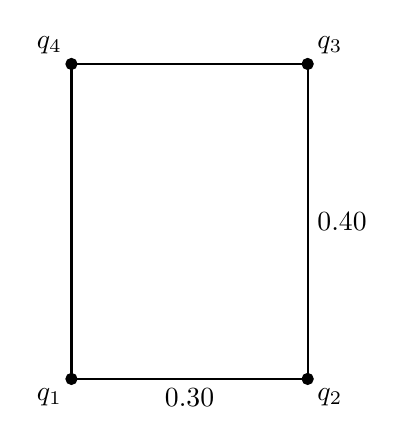
\begin{tikzpicture}[scale=1]

\coordinate (A) at (0,0);
\coordinate (B) at (3,0);
\coordinate (C) at (3,4);
\coordinate (D) at (0,4);

\draw[thick] (A) -- (B) -- (C) -- (D) -- cycle;

\filldraw (A) circle (2pt) node[below left] {$q_1$};
\filldraw (B) circle (2pt) node[below right] {$q_2$};
\filldraw (C) circle (2pt) node[above right] {$q_3$};
\filldraw (D) circle (2pt) node[above left] {$q_4$};

\node[below] at (1.5,0) {\(\SI{0.30}{\metre}\)};
\node[right] at (3,2) {\(\SI{0.40}{\metre}\)};

\end{tikzpicture}
\end{center}

Determine la energía potencial eléctrica total.

\end{ejercicio}

\begin{respuesta}

\[
\boxed{U\approx-\SI{0.246}{\joule}}
\]

\end{respuesta}

\begin{explicacion}

Existen seis pares diferentes.

Las distancias son

\[
r_{12}=r_{34}=\SI{0.30}{\metre},
\]

\[
r_{14}=r_{23}=\SI{0.40}{\metre},
\]

y las diagonales valen

\[
r_{13}=r_{24}
=
\sqrt{(0.30)^2+(0.40)^2}
=
\SI{0.50}{\metre}.
\]

Calculamos cada interacción:

\[
U_{12}
=
k\frac{q_1q_2}{r_{12}}
\approx-\SI{0.1199}{\joule},
\]

\[
U_{13}
=
k\frac{q_1q_3}{r_{13}}
\approx+\SI{0.1079}{\joule},
\]

\[
U_{14}
=
k\frac{q_1q_4}{r_{14}}
\approx-\SI{0.0450}{\joule},
\]

\[
U_{23}
=
k\frac{q_2q_3}{r_{23}}
\approx-\SI{0.1349}{\joule},
\]

\[
U_{24}
=
k\frac{q_2q_4}{r_{24}}
\approx+\SI{0.0360}{\joule},
\]

\[
U_{34}
=
k\frac{q_3q_4}{r_{34}}
\approx-\SI{0.0899}{\joule}.
\]

La energía total es

\[
U
=
U_{12}+U_{13}+U_{14}+U_{23}+U_{24}+U_{34}.
\]

Entonces,

\[
\boxed{U\approx-\SI{0.246}{\joule}}.
\]

\end{explicacion}


\begin{ejercicio}

Tres cargas están sobre el eje \(x\):

\[
q_1=+q
\quad\text{en}\quad x=0,
\]

\[
q_2
\quad\text{en}\quad x=a,
\]

\[
q_3=+q
\quad\text{en}\quad x=2a.
\]

Determine \(q_2\) para que la energía potencial eléctrica total del sistema sea cero.

\end{ejercicio}

\begin{respuesta}

\[
\boxed{q_2=-\frac{q}{4}}
\]

\end{respuesta}

\begin{explicacion}

Las distancias son

\[
r_{12}=a,
\qquad
r_{23}=a,
\qquad
r_{13}=2a.
\]

La energía total es

\[
U
=
k
\left(
\frac{qq_2}{a}
+
\frac{q_2q}{a}
+
\frac{q^2}{2a}
\right).
\]

Factorizamos:

\[
U
=
\frac{k}{a}
\left(
2qq_2+\frac{q^2}{2}
\right).
\]

Imponemos

\[
U=0.
\]

Entonces,

\[
2qq_2+\frac{q^2}{2}=0.
\]

Dividiendo entre \(q\),

\[
2q_2+\frac{q}{2}=0.
\]

Por tanto,

\[
\boxed{q_2=-\frac{q}{4}}.
\]

\end{explicacion}


\begin{ejercicio}

Una carga fija

\[
Q=+\SI{3.0}{\micro\coulomb}
\]

atrae a una partícula de carga

\[
q=-\SI{2.0}{\micro\coulomb}
\]

y masa

\[
m=\SI{4.0e-3}{\kilogram}.
\]

La partícula se encuentra inicialmente a una distancia

\[
r_i=\SI{0.20}{\metre}.
\]

Determine la rapidez mínima que debe recibir dirigida radialmente hacia afuera para
que pueda alejarse hasta el infinito con rapidez final nula.

\end{ejercicio}

\begin{respuesta}

\[
\boxed{v_{\min}\approx\SI{11.6}{\metre\per\second}}
\]

\end{respuesta}

\begin{explicacion}

Para que la partícula llegue al infinito con rapidez final nula,

\[
K_f=0,
\qquad
U_f=0.
\]

Por conservación de la energía,

\[
K_i+U_i=0.
\]

La energía potencial inicial es

\[
U_i
=
k\frac{Qq}{r_i}.
\]

Sustituyendo,

\[
U_i
=
(8.99\times10^9)
\frac{(3.0\times10^{-6})(-2.0\times10^{-6})}{0.20}
=
-\SI{0.2697}{\joule}.
\]

Por tanto,

\[
K_i=\SI{0.2697}{\joule}.
\]

Como

\[
K_i=\frac12mv_{\min}^2,
\]

tenemos

\[
v_{\min}
=
\sqrt{
\frac{2(0.2697)}
{4.0\times10^{-3}}
}.
\]

Así,

\[
\boxed{v_{\min}\approx\SI{11.6}{\metre\per\second}}.
\]

Una rapidez menor no proporcionaría suficiente energía para alcanzar una separación
infinita.

\end{explicacion}


\begin{ejercicio}

En la situación del ejercicio anterior, la partícula recibe una rapidez inicial de

\[
v_i=\SI{8.0}{\metre\per\second}
\]

dirigida radialmente hacia afuera.

Determine la máxima distancia que alcanzará antes de regresar hacia la carga positiva.

\end{ejercicio}

\begin{respuesta}

\[
\boxed{r_{\max}\approx\SI{0.381}{\metre}}
\]

\end{respuesta}

\begin{explicacion}

La energía potencial inicial es

\[
U_i=-\SI{0.2697}{\joule}.
\]

La energía cinética inicial es

\[
K_i
=
\frac12mv_i^2
=
\frac12(4.0\times10^{-3})(8.0)^2.
\]

Entonces,

\[
K_i=\SI{0.128}{\joule}.
\]

La energía mecánica total es

\[
E_{\text{mec}}
=
K_i+U_i.
\]

Así,

\[
E_{\text{mec}}
=
0.128-0.2697
=
-\SI{0.1417}{\joule}.
\]

En la máxima separación la partícula se detiene momentáneamente:

\[
K_f=0.
\]

Por tanto,

\[
U_f=E_{\text{mec}}.
\]

Entonces,

\[
k\frac{Qq}{r_{\max}}
=
-\SI{0.1417}{\joule}.
\]

Como

\[
kQq
=
(8.99\times10^9)
(3.0\times10^{-6})(-2.0\times10^{-6}),
\]

despejamos

\[
r_{\max}
=
\frac{kQq}{E_{\text{mec}}}.
\]

Los dos valores son negativos, por lo que la distancia resulta positiva:

\[
r_{\max}
\approx
\SI{0.381}{\metre}.
\]

Por tanto,

\[
\boxed{r_{\max}\approx\SI{0.381}{\metre}}.
\]

La energía mecánica total es negativa, por lo que la partícula no posee suficiente
energía para escapar hasta el infinito.

\end{explicacion}